% Created by tikzDevice version 0.5.2 on 2011-03-14 15:14:43
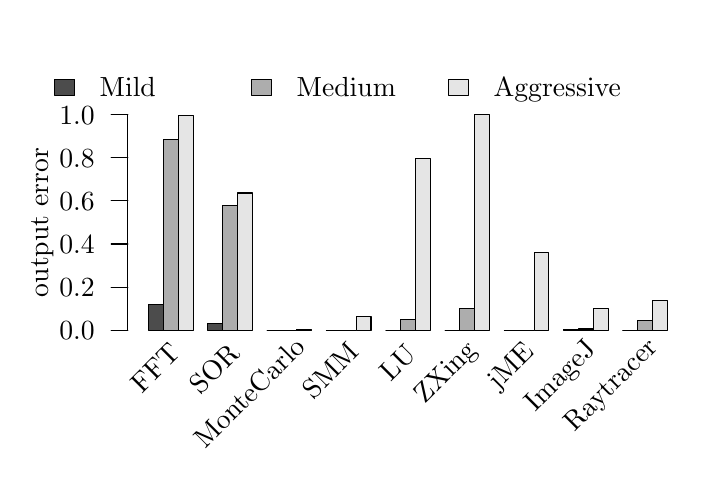
\begin{tikzpicture}[x=1pt,y=1pt]
\draw[color=white,opacity=0] (0,0) rectangle (238.49,151.77);
\begin{scope}
\path[clip] (  0.00,  0.00) rectangle (238.49,151.77);
\definecolor[named]{drawColor}{rgb}{0.18,0.00,0.42}
\definecolor[named]{fillColor}{rgb}{0.45,0.45,0.18}
\definecolor[named]{drawColor}{rgb}{0.00,0.00,0.00}
\definecolor[named]{fillColor}{rgb}{0.30,0.30,0.30}

\draw[color=drawColor,line cap=round,line join=round,fill=fillColor,] ( 43.50, 42.60) rectangle ( 48.86, 51.92);
\definecolor[named]{fillColor}{rgb}{0.68,0.68,0.68}

\draw[color=drawColor,line cap=round,line join=round,fill=fillColor,] ( 48.86, 42.60) rectangle ( 54.21,111.42);
\definecolor[named]{fillColor}{rgb}{0.90,0.90,0.90}

\draw[color=drawColor,line cap=round,line join=round,fill=fillColor,] ( 54.21, 42.60) rectangle ( 59.57,120.23);
\definecolor[named]{fillColor}{rgb}{0.30,0.30,0.30}

\draw[color=drawColor,line cap=round,line join=round,fill=fillColor,] ( 64.93, 42.60) rectangle ( 70.28, 45.09);
\definecolor[named]{fillColor}{rgb}{0.68,0.68,0.68}

\draw[color=drawColor,line cap=round,line join=round,fill=fillColor,] ( 70.28, 42.60) rectangle ( 75.64, 87.67);
\definecolor[named]{fillColor}{rgb}{0.90,0.90,0.90}

\draw[color=drawColor,line cap=round,line join=round,fill=fillColor,] ( 75.64, 42.60) rectangle ( 81.00, 92.21);
\definecolor[named]{fillColor}{rgb}{0.30,0.30,0.30}

\draw[color=drawColor,line cap=round,line join=round,fill=fillColor,] ( 86.35, 42.60) rectangle ( 91.71, 42.60);
\definecolor[named]{fillColor}{rgb}{0.68,0.68,0.68}

\draw[color=drawColor,line cap=round,line join=round,fill=fillColor,] ( 91.71, 42.60) rectangle ( 97.07, 42.61);
\definecolor[named]{fillColor}{rgb}{0.90,0.90,0.90}

\draw[color=drawColor,line cap=round,line join=round,fill=fillColor,] ( 97.07, 42.60) rectangle (102.43, 42.85);
\definecolor[named]{fillColor}{rgb}{0.30,0.30,0.30}

\draw[color=drawColor,line cap=round,line join=round,fill=fillColor,] (107.78, 42.60) rectangle (113.14, 42.60);
\definecolor[named]{fillColor}{rgb}{0.68,0.68,0.68}

\draw[color=drawColor,line cap=round,line join=round,fill=fillColor,] (113.14, 42.60) rectangle (118.50, 42.60);
\definecolor[named]{fillColor}{rgb}{0.90,0.90,0.90}

\draw[color=drawColor,line cap=round,line join=round,fill=fillColor,] (118.50, 42.60) rectangle (123.85, 47.53);
\definecolor[named]{fillColor}{rgb}{0.30,0.30,0.30}

\draw[color=drawColor,line cap=round,line join=round,fill=fillColor,] (129.21, 42.60) rectangle (134.57, 42.60);
\definecolor[named]{fillColor}{rgb}{0.68,0.68,0.68}

\draw[color=drawColor,line cap=round,line join=round,fill=fillColor,] (134.57, 42.60) rectangle (139.92, 46.64);
\definecolor[named]{fillColor}{rgb}{0.90,0.90,0.90}

\draw[color=drawColor,line cap=round,line join=round,fill=fillColor,] (139.92, 42.60) rectangle (145.28,104.67);
\definecolor[named]{fillColor}{rgb}{0.30,0.30,0.30}

\draw[color=drawColor,line cap=round,line join=round,fill=fillColor,] (150.64, 42.60) rectangle (155.99, 42.60);
\definecolor[named]{fillColor}{rgb}{0.68,0.68,0.68}

\draw[color=drawColor,line cap=round,line join=round,fill=fillColor,] (155.99, 42.60) rectangle (161.35, 50.40);
\definecolor[named]{fillColor}{rgb}{0.90,0.90,0.90}

\draw[color=drawColor,line cap=round,line join=round,fill=fillColor,] (161.35, 42.60) rectangle (166.71,120.57);
\definecolor[named]{fillColor}{rgb}{0.30,0.30,0.30}

\draw[color=drawColor,line cap=round,line join=round,fill=fillColor,] (172.07, 42.60) rectangle (177.42, 42.60);
\definecolor[named]{fillColor}{rgb}{0.68,0.68,0.68}

\draw[color=drawColor,line cap=round,line join=round,fill=fillColor,] (177.42, 42.60) rectangle (182.78, 42.60);
\definecolor[named]{fillColor}{rgb}{0.90,0.90,0.90}

\draw[color=drawColor,line cap=round,line join=round,fill=fillColor,] (182.78, 42.60) rectangle (188.14, 70.78);
\definecolor[named]{fillColor}{rgb}{0.30,0.30,0.30}

\draw[color=drawColor,line cap=round,line join=round,fill=fillColor,] (193.49, 42.60) rectangle (198.85, 42.85);
\definecolor[named]{fillColor}{rgb}{0.68,0.68,0.68}

\draw[color=drawColor,line cap=round,line join=round,fill=fillColor,] (198.85, 42.60) rectangle (204.21, 43.07);
\definecolor[named]{fillColor}{rgb}{0.90,0.90,0.90}

\draw[color=drawColor,line cap=round,line join=round,fill=fillColor,] (204.21, 42.60) rectangle (209.56, 50.54);
\definecolor[named]{fillColor}{rgb}{0.30,0.30,0.30}

\draw[color=drawColor,line cap=round,line join=round,fill=fillColor,] (214.92, 42.60) rectangle (220.28, 42.61);
\definecolor[named]{fillColor}{rgb}{0.68,0.68,0.68}

\draw[color=drawColor,line cap=round,line join=round,fill=fillColor,] (220.28, 42.60) rectangle (225.63, 46.15);
\definecolor[named]{fillColor}{rgb}{0.90,0.90,0.90}

\draw[color=drawColor,line cap=round,line join=round,fill=fillColor,] (225.63, 42.60) rectangle (230.99, 53.23);
\end{scope}
\begin{scope}
\path[clip] (  0.00,  0.00) rectangle (238.49,151.77);
\definecolor[named]{drawColor}{rgb}{0.18,0.00,0.42}
\definecolor[named]{fillColor}{rgb}{0.45,0.45,0.18}
\definecolor[named]{drawColor}{rgb}{0.00,0.00,0.00}

\draw[color=drawColor,line cap=round,line join=round,fill opacity=0.00,] ( 36.00, 42.60) -- ( 36.00,120.57);

\draw[color=drawColor,line cap=round,line join=round,fill opacity=0.00,] ( 36.00, 42.60) -- ( 30.00, 42.60);

\draw[color=drawColor,line cap=round,line join=round,fill opacity=0.00,] ( 36.00, 58.19) -- ( 30.00, 58.19);

\draw[color=drawColor,line cap=round,line join=round,fill opacity=0.00,] ( 36.00, 73.79) -- ( 30.00, 73.79);

\draw[color=drawColor,line cap=round,line join=round,fill opacity=0.00,] ( 36.00, 89.38) -- ( 30.00, 89.38);

\draw[color=drawColor,line cap=round,line join=round,fill opacity=0.00,] ( 36.00,104.97) -- ( 30.00,104.97);

\draw[color=drawColor,line cap=round,line join=round,fill opacity=0.00,] ( 36.00,120.57) -- ( 30.00,120.57);

\node[color=drawColor,anchor=base east,inner sep=0pt, outer sep=0pt, scale=  1.00] at ( 24.00, 39.16) {0.0%
};

\node[color=drawColor,anchor=base east,inner sep=0pt, outer sep=0pt, scale=  1.00] at ( 24.00, 54.75) {0.2%
};

\node[color=drawColor,anchor=base east,inner sep=0pt, outer sep=0pt, scale=  1.00] at ( 24.00, 70.34) {0.4%
};

\node[color=drawColor,anchor=base east,inner sep=0pt, outer sep=0pt, scale=  1.00] at ( 24.00, 85.94) {0.6%
};

\node[color=drawColor,anchor=base east,inner sep=0pt, outer sep=0pt, scale=  1.00] at ( 24.00,101.53) {0.8%
};

\node[color=drawColor,anchor=base east,inner sep=0pt, outer sep=0pt, scale=  1.00] at ( 24.00,117.12) {1.0%
};

\node[rotate= 90.00,color=drawColor,anchor=base,inner sep=0pt, outer sep=0pt, scale=  1.00] at (  7.20, 81.58) {output error%
};
\end{scope}
\begin{scope}
\path[clip] (  0.00,  0.00) rectangle (238.49,151.77);
\definecolor[named]{drawColor}{rgb}{0.18,0.00,0.42}
\definecolor[named]{fillColor}{rgb}{0.45,0.45,0.18}
\definecolor[named]{drawColor}{rgb}{0.00,0.00,0.00}
\definecolor[named]{fillColor}{rgb}{0.30,0.30,0.30}

\draw[color=drawColor,line cap=round,line join=round,fill=fillColor,] (  9.64,133.40) rectangle ( 16.84,127.40);
\definecolor[named]{fillColor}{rgb}{0.68,0.68,0.68}

\draw[color=drawColor,line cap=round,line join=round,fill=fillColor,] ( 80.81,133.40) rectangle ( 88.01,127.40);
\definecolor[named]{fillColor}{rgb}{0.90,0.90,0.90}

\draw[color=drawColor,line cap=round,line join=round,fill=fillColor,] (151.97,133.40) rectangle (159.17,127.40);

\node[color=drawColor,anchor=base west,inner sep=0pt, outer sep=0pt, scale=  1.00] at ( 25.84,126.95) {Mild%
};

\node[color=drawColor,anchor=base west,inner sep=0pt, outer sep=0pt, scale=  1.00] at ( 97.01,126.95) {Medium%
};

\node[color=drawColor,anchor=base west,inner sep=0pt, outer sep=0pt, scale=  1.00] at (168.17,126.95) {Aggressive%
};

\node[rotate= 45.00,color=drawColor,anchor=base east,inner sep=0pt, outer sep=0pt, scale=  1.00] at ( 55.40, 33.80) {FFT%
};

\node[rotate= 45.00,color=drawColor,anchor=base east,inner sep=0pt, outer sep=0pt, scale=  1.00] at ( 76.86, 33.83) {SOR%
};

\node[rotate= 45.00,color=drawColor,anchor=base east,inner sep=0pt, outer sep=0pt, scale=  1.00] at (100.48, 36.02) {MonteCarlo%
};

\node[rotate= 45.00,color=drawColor,anchor=base east,inner sep=0pt, outer sep=0pt, scale=  1.00] at (119.94, 34.06) {SMM%
};

\node[rotate= 45.00,color=drawColor,anchor=base east,inner sep=0pt, outer sep=0pt, scale=  1.00] at (140.65, 33.34) {LU%
};

\node[rotate= 45.00,color=drawColor,anchor=base east,inner sep=0pt, outer sep=0pt, scale=  1.00] at (162.33, 34.96) {ZXing%
};

\node[rotate= 45.00,color=drawColor,anchor=base east,inner sep=0pt, outer sep=0pt, scale=  1.00] at (183.19, 34.40) {jME%
};

\node[rotate= 45.00,color=drawColor,anchor=base east,inner sep=0pt, outer sep=0pt, scale=  1.00] at (205.50, 35.28) {ImageJ%
};

\node[rotate= 45.00,color=drawColor,anchor=base east,inner sep=0pt, outer sep=0pt, scale=  1.00] at (227.74, 36.09) {Raytracer%
};
\end{scope}
\end{tikzpicture}
